\begin{figure}
	\center
	\begin{minipage}{0.49\linewidth}
		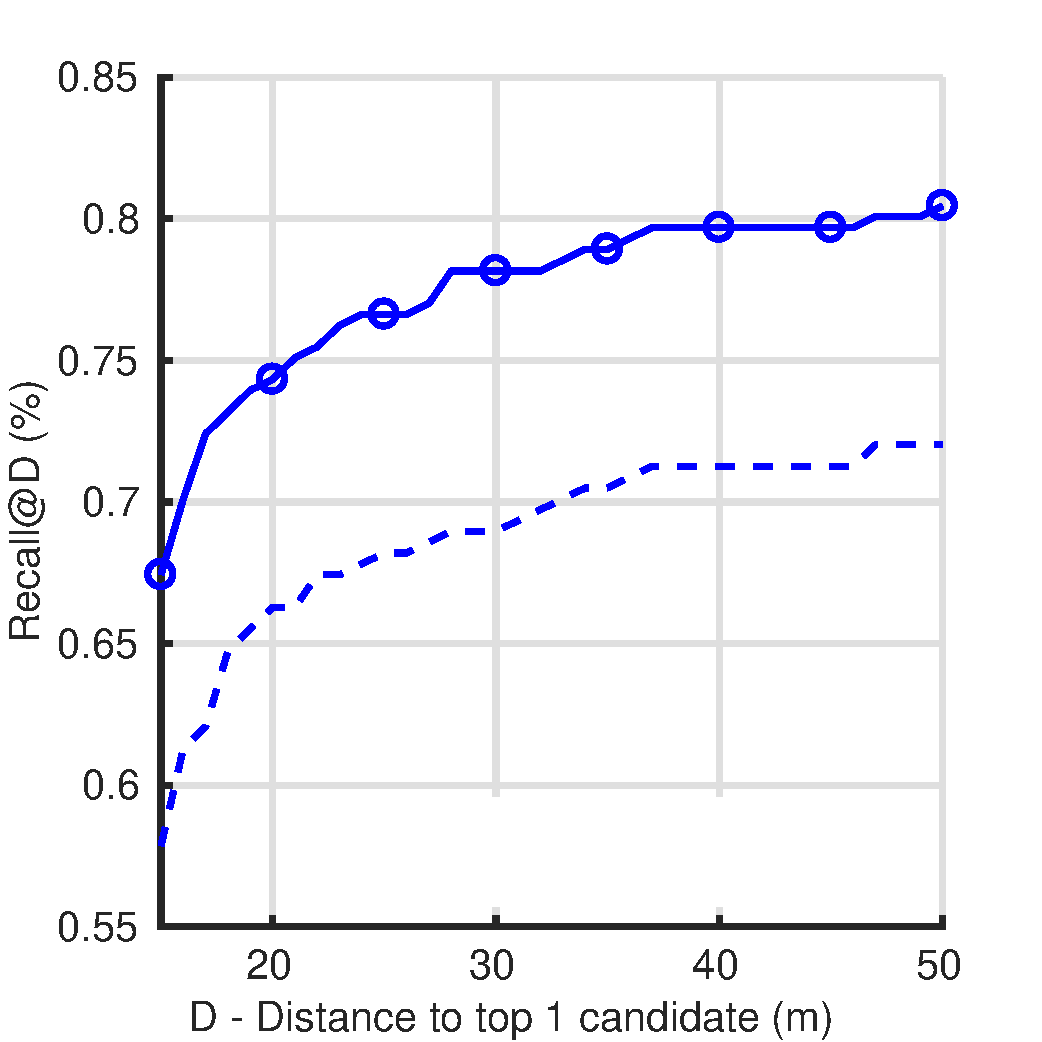
\includegraphics[width=\linewidth]{plot/full_vs_trunc/rgb_r_trunc_distance}	
	\end{minipage}
	\begin{minipage}{0.49\linewidth}
		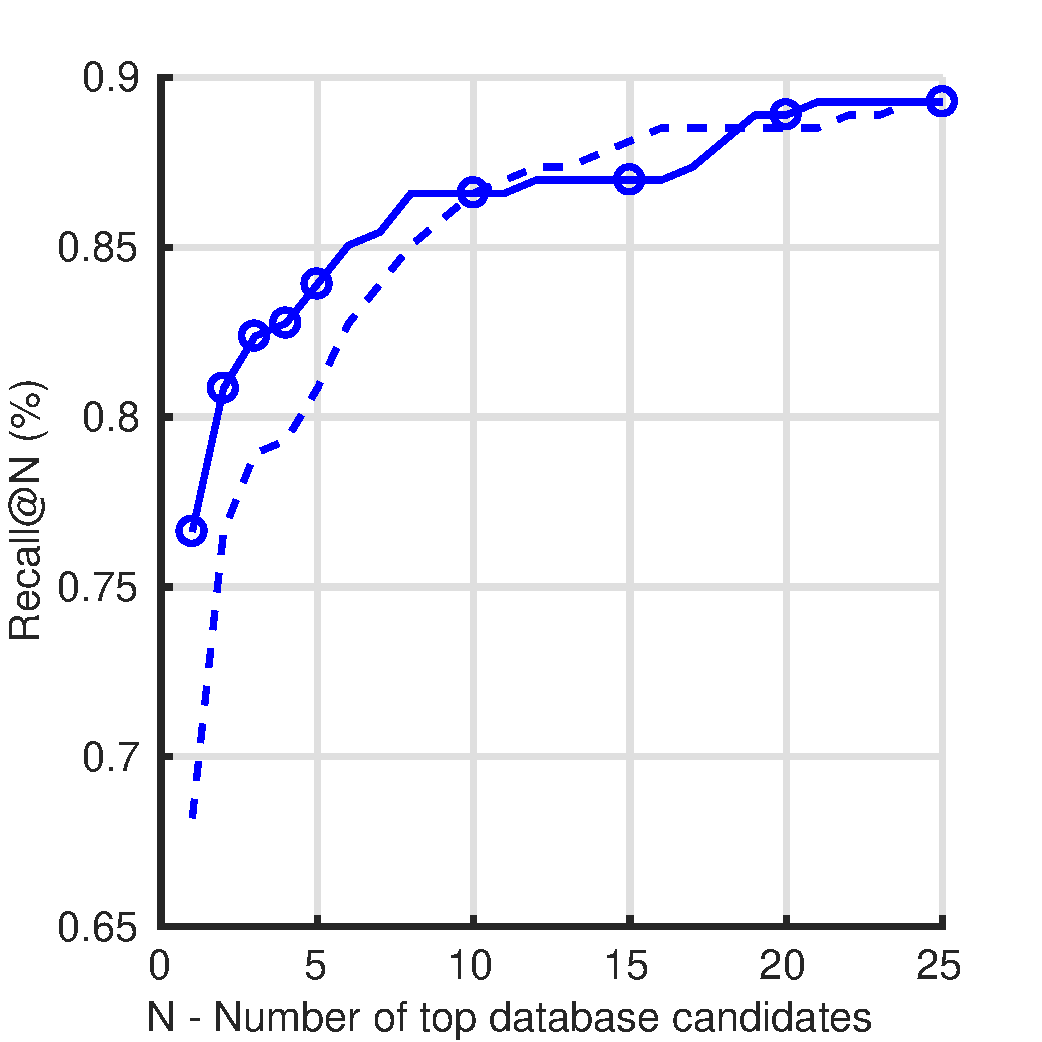
\includegraphics[width=\linewidth]{plot/full_vs_trunc/rgb_r_trunc_recall}	
	\end{minipage}
	
	\vspace{0.2cm}
	
	\begin{scriptsize}
	\begin{tabular}{c c c c}
		\textcolor{blue}{\large{- -}} & R + NetVALD & \textcolor{blue}{\large{$\mathclap{\circ} \mathclap{-}$}} & Rt + NetVALD \\
	\end{tabular}		
	\end{scriptsize}

	\caption{\label{fig:trunc_resnet} \textbf{Resnet18 (R) versus truncated Resnet18 (Rt) in combination with NetVLAD pooling:} we show the importance of the spatial resolution of the deep feature maps of the encoder used with NetVLAD layer. The truncated version of Resnet18, more than two times lighter than the complete one, achieves much better localization results.}
\end{figure}